%%% -*-LaTeX-*-

\chapter{Graphs for Data Analysis}
\label{ch:graphs}

\DPM{This chapter is largely a work in progress.}

\section{The $\beta_p$-Skeleton}
\label{sec:bpskeleton}
Let us begin with a formal definition of the lune-based $\beta$-skeleton.
%
First, define an open $p$-ball, $B$ of radius $r$ centered at some point $c$ in $d$-dimensions to be:

\begin{equation}
\label{eq:ball}
    B_{r,p}(c) = \{x \in \mathbb{R}^d : || x  - c ||_p < r\}
\end{equation}

In previous literature, typically $p$ is set to $2$.
%
Given two points $a$ and $b$, their $L^2$ distance $l_{ab}$, and a $\beta$ parameter, we can define a radius $r$ as:

\begin{equation}
    \label{eq:beta_radius}
    r =
    \begin{cases}
        \frac{l_{ab}}{2\beta}, & \text{if $0 < \beta < 1$}.\\
        \frac{l_{ab}\beta}{2}, & \text{otherwise}.
    \end{cases}
\end{equation}

This allows us to now define the region for the edge $ab$ as follows:

\begin{equation}
    R_{\beta,p}(a,b) = \left(\bigcap_{c \in C} B_{r,p}(c)\right)
\end{equation}

Where $C$ is the set of points equidistant to both $a$ and $b$:

\begin{equation}
    C = \{c \in \mathbb{R}^d: ||a -c||_2 = ||b - c||_2 = r\}
\end{equation}

Formally, we extend the existing empty region definition by considering various $p$ values in Equation~\ref{eq:ball}.
%
Note, $p$ modulates the \emph{shape} of the balls whereas $\beta$ controls the \emph{size} of the balls.
%
This allows us to evaluate the performance of an entire spectrum of different values representing graphs we have not seen before in the context of known graphs.

\begin{figure}
    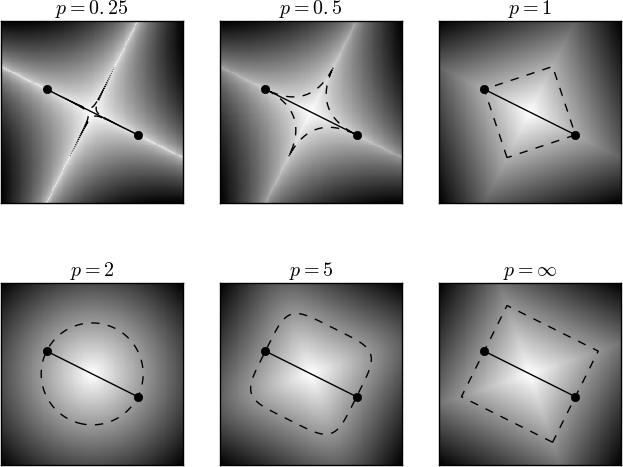
\includegraphics[width=\linewidth]{figs/chap7/emptyRegions}
    \caption{The generalization of the Gabriel graph ($\beta$-skeleton where $\beta=1$) using balls defined under different $p$-norms.
    %
    Here we show a graph edge as a solid black line joining two vertices.
    %
    The boundary of the empty region is noted by the dashed line in each example.
    %
    This line is a levelset ($f(c)=1$) of the $p$-norm from the midpoint of the edge.
    %
    The grayscale map denotes this function.
    %
    Note, how the shape of the region varies from a Dirac delta function ($p \rightarrow 0$) to concave to convex to a square in the limit ($p \rightarrow \infty$).}
    \label{fig:gabriel_p_shapes}
\end{figure}

From the definition above, we see that the empty regions of the $\beta$-skeleton can be viewed as the intersection of all balls defined under some metric centered equidistantly from the proposed edge's midpoint.
%
The introduced $p$ parameter defines the $p$-norm to use as the metric.
%
Our generalization allows us to still compute both strict and relaxed versions of our graphs~\cite{CorreaLindstrom2011}.
%
One caveat with our GPU implementation outlined in Section~\ref{sec:method} is that we only consider \textit{symmetric} graphs and not \textit{mutual} versions as defined by Correa and Lindstrom~\cite{CorreaLindstrom2011}.

\section{Approximate Cone Graphs for High-Dimensional Analysis}

A major challenge of working with cone-based graphs is in the generation of equally-sized high-dimensional cones.
%
In order to do this, we first note that we actually only require the axes of said cones and not the interiors or boundaries.
%
Secondly, the orientation of these cones is not prescribed in any prior work, so any set of uniformly spaced rays emanating from a point will suffice.
%
To do this, we utilize a constrained centroidal Voronoi tessellation (CCVT) algorithm to generate approximately equally spaced directions in high dimensions~\cite{DuGunzburgerJu2003}.
%
\DPM{Hesse et al.~\cite{HesseSlaonWomersley2015} claim a CVT is an equal area partition, but the only
guarantee with a CVT sampling is that the centers of mass align with the Voronoi sites.}
%
\DPM{Also exploring the use of Poisson disk sampling for this.}
%
Specifically, we constrain a CVT sampling to the surface of a $d$-dimensional unit hypersphere.
%
By drawing vectors from the origin to these surface points, we generate a set of roughly equally spaced directions that can be used as the axes of the approximately equally sized hypercones.
%
In our GPU framework introduced in Section~\ref{sec:gpu_graphs}, these directions can be computed once and reused for every point query on the GPU.
%
Alternatively, we can utilize the dependence on the random seed points to generate several different realizations.
%
This fact will be exploited to create probabilistic cone-based graphs.

We make the claim that the CCVT sampling will generate roughly equal cones with no formal proof.
%
In lieu of a formal proof, we performed a study where we estimate the surface area of each CCVT sample's Voronoi region on the hypersphere by performing Monte Carlo sampling on the surface of the hypersphere.
%
By associating every surface point to its nearest site, we can construct a histogram for the sites' count of constituent points.
%
The results are summarized in Figure~\ref{fig:cvt_study}.
%
A 2D example CCVT sample set is shown in the left image with the surface points colored by their membership.
%
The histogram of the middle image shows the frequency of labels for each CCVT site.
%
The black dotted line represent the expected value.
%
The right two line plots summarize our results across dimensions and increasing cone counts.
%
Interestingly enough, we do not see performance degrade as we increase dimensionality, although we do see it degrade as we increase the number of cones.

\begin{figure}
    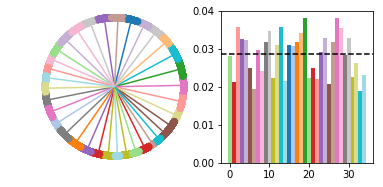
\includegraphics[width=0.65\linewidth]{figs/chap7/cvt_study_35.png}
    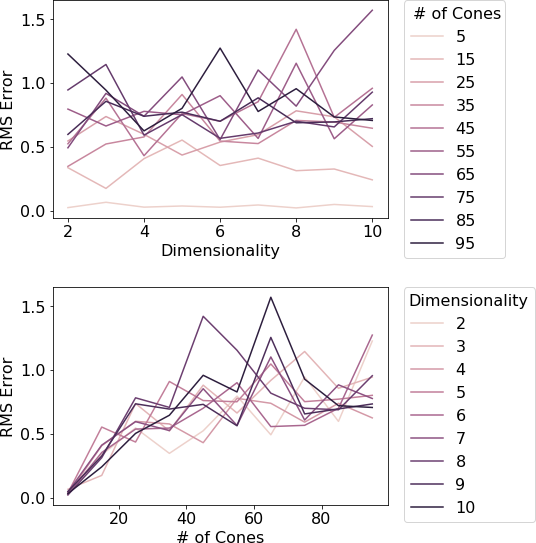
\includegraphics[width=0.32\linewidth]{figs/chap7/scvt.png}
    \caption{A study of the relative areas of Constrained CVT samples indicates that their error, although non-zero, is within tolerance for the examples we consider.
    %
    Left: an example CCVT sample showing point membership is used for visual inspection of quality.
    %
    Middle: A histogram showing the membership counts of each site.
    %
    Top Right: We summarize the root mean square as a function of the dimensionality.
    %
    Bottom right: We summarize the root mean square error as a function of the number of cones requested.}
    \label{fig:cvt_study}
\end{figure}

Generally, the number of directions or cones, $c$, should be much smaller than the $k$ value in order to effectively prune redundant directions, but it will also depend on the dimensionality, $d$, of the data.
%
This is also advantageous since our approximation is more accurate with smaller values of $c$.

\section{A Unified GPU Framework}
\label{sec:gpu_graphs}

The NGL library~\cite{CorreaLindstrom2011} is an efficient serial implementation able to build $\beta$-skeleton and diamond graphs and their corresponding relaxed versions on arbitrary dimensional datasets.
%
Efficiency is achieved by relaxing the strict requirement of testing all possible edges with all possible points, and thus should be considered an approximation to the true empty region graphs.
%
Even so, the serial implementation of NGL only scales so far on commodity hardware, and as performance improvements are continuously made on the underlying data structures such as the $k$-nearest neighbor graph discussed below, the empty region test remains the bottleneck of this implementation.
%
Our GPU-parallel implementation is a simple extension of the technique used by NGL with a few added generalities to allow for the computation of a more robust collection of graphs.
%
In addition, we formulate probabilistic versions of these graphs that are also amenable to the GPU.
%
Our algorithms rely on the same data structures as NGL and thus should be considered approximations to the true graphs.
%
Rather than building graphs incrementally by testing and keeping individual edges, all techniques described from here on will instead prune a supergraph by testing properties of edges in the supergraph and removing those that fail an \emph{edge test} condition.

Both NGL and our proposed method employ an approximate $k$-nearest neighbor structure to speed up edge testing.
%
Evaluating different implementations of $k$-nn approximations is beyond the scope of this paper however we have built a library that is compatible with several of the leading $k$-nn implementations as demonstrated in a recent benchmark~\cite{AumullerBernhardssonFaithfull2017}.
%
Edge testing is limited by only considering edges that exist in the $k$-nn graph.
%
Furthermore, when performing edge tests, we only consider points that are in the $k$-nearest neighborhood of either endpoint.
%
When using this data structure, $k$ is typically set to a large enough value so as to not drastically affect the resulting computation.
%
% Note, we address the setting of $k$ and the effect on approximation quality over different datasets with a study in Section~\ref{exp:approximation}.

In this setting, we assume a $k$-nearest neighbor index is available that is able to efficiently return the $k$ nearest neighbors in sorted order for one ore more query points in our data set.
%
Thus far, we have $n \times d$ floating point values representing the locations of a $d$-dimensional point set of size $n$ plus $n \times k$ integers representing the $k$ nearest indices for each of our $n$ points which must be moved to the GPU for edge validity testing.
%
We then parallelize the pruning operation by associating individual GPU threads to distinct points in the data set.
%
For each thread/point, we iteratively perform the edge test on each of its neighbors.
%
Thus, each of $n$ threads will perform $k$ edge tests.

For smaller datasets, we can fit the entire $n \times d$ dataset plus its $n \times k$ graph on GPU RAM, and thus we can trivially parallelize the problem using the method described.
%
However, for larger datasets or GPUs with less available memory, we must move part of the problem onto the GPU at a time and process the data in chunks and return the results.
%
Let us consider such a problem, where $b$ is the batch size of points we can process in parallel on the GPU.
%
For simplicity, we utilize a fixed batch size determined by the worst case analysis for the different graphs.
%
In the partial case, we do not want to move the entire point set, but rather only the set of information required for testing.
%
This is where our methodology diverges depending on the graph selected.

For cone-based graphs and relaxed $\beta$-skeletons we only need location information for the points we are pruning and all of their neighbors.
%
In the worst case, each of our $b$ points could each have $k$ distinct neighbors, thus we require storage of $bkd$ floating point location values.
%
Additionally, we require the indices of the neighboring points mapped to the subset of the location data which is an additional $bk$ integer index values.
%
From this analysis, we can determine the largest batch size able to fit into our GPU memory:

\begin{equation}
    bkds_{float} + bks_{int} \leq M_{GPU}
\end{equation}

Where $M_{GPU}$ is the total amount of memory avaiable on our device (in bytes), and $s_{float}$ and $s_{int}$ are the sizes of floats and ints (in bytes), respectively.
%
Solving for $b$ results in the following equation:

\begin{equation}
    b \leq \frac{M_{GPU}}{k(ds_{float} + s_{int})}
\end{equation}

The analysis for the strict $\beta$-skeletons requires care as we need not only the locations of the points and their neighbors, but also all of their neighbors' neighbors.
%
In the worst case, every neighbor could contribute $k$ points yet unseen in our working subset resulting in $bkd$ floating point values describing the locations of the query points and all of their neighbors plus an additional $bk^2d$ floating points for the potential $k^2$ neighbors of neighbors.
%
Additionally, we require storing mapped integer indices to this subset of data to represent the neighborhoods.
%
In this case, we have $b$ query points with $k$ neighbors each plus we need the $k$ neighbors of each of those neighbors.
%
The result is $b(k + k^2)$ integer values.
%
In summary, the available batch size for the strict $\beta$-skeletons on a device with $M_{GPU}$ bytes of free memory is given below:

\begin{equation}
    b \leq \frac{M_{GPU}}{(k+k^2)\left(ds_{float} + s_{int}\right)}
\end{equation}

This affords much less parallelism and one should consider moving to an adaptive scheme and/or possibly sorting data points based on their location in order to batch nearby query points together to avoid this worst case upper bound when using the strict $\beta$-skeleton.
%
We instead focus our attention on comparing the relative performance of the relaxed and strict versions algorithm in order to make a case that for many practical purposes the relaxed $\beta$-skeletons are ``good enough.''

% \dpm{For our $6$GB test machine working up to $5$D with a $k=1024$ and assuming $s_{float} = s_{int} = 4$, we can still achieve parallelism with a batch size of $238$, however with a relaxed $\beta$-skeleton or a cone-graph we can achieve $b=244140$}

\subsection{Empty Region Graphs}
We begin with an observation that the empty region shapes defined by any particular $\beta_p$-skeleton are symmetric in all directions orthogonal to an edge regardless of the dimensionality of the embedding space of the edge.
%
Thus, we can reduce all point in empty region tests to a one-dimensional problem.
%
This is done by defining the edge as a directed vector, say from point $a$ to point $b$.
%
We then form vectors to every $k$ nearest neighbor, $q$, of $a$ (and $b$, if computing the strict version of the graph).
%
Every vector $aq$ is projected onto $ab$ using a dot product which yields a parameterization of $t_q$.
%
Note, the maximal shape any lune-based $\beta_p$-skeleton can attain is the infinite slab of space bounded by two hyperplanes, each one intersecting one endpoint and perpendicular to the edge.
%
An example of this region is shown by the shaded region in the left image of Figure~\ref{fig:infinite_slab} for the two-dimensional case.
%
This means that only points that have a $t$ value on the range $(0,1)$ can possibly intersect the empty region.
%
For the neighbors whose $t_q \in (0,1)$, we compute the $L^2$-norm from $q$ to the edge and compare it with the empty region.

\begin{figure}
    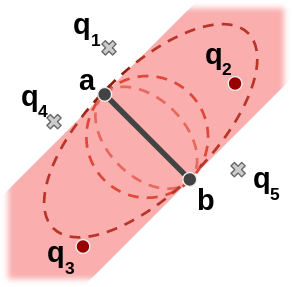
\includegraphics[width=0.34\linewidth]{figs/chap7/infinite_slab.png}
    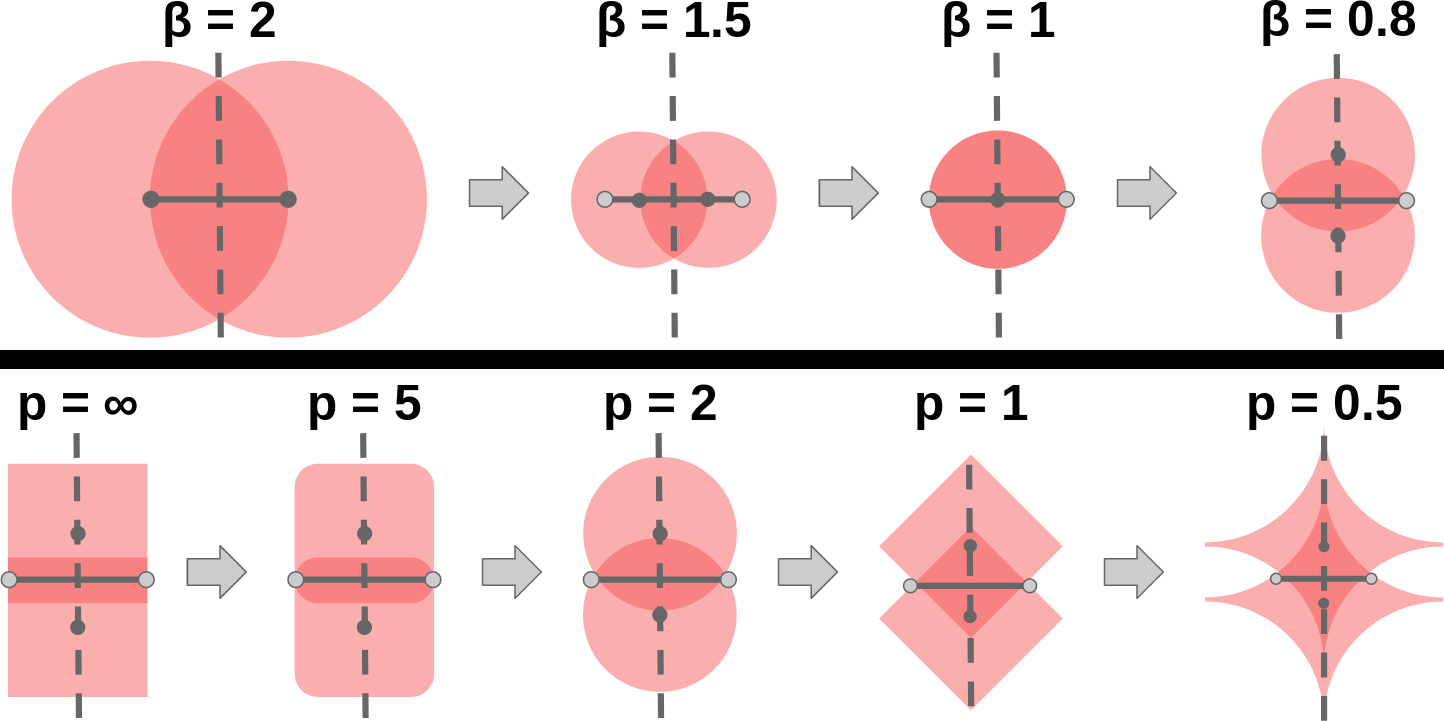
\includegraphics[width=0.64\linewidth]{figs/chap7/variable_parameters.png}
    \caption{Left: Consider an edge between points $a$ and $b$ and neighbors to $a$, $q_{i}$.
    %
    The shaded region represents $R$ for the infinite slab graph ($p < 1, \beta \rightarrow 0$).
    %
    All other parameterizations of the $\beta_p$-skeleton will yield subsets of this region.
    %
    Dotted curves represent the empty regions of other parameterizations.
    %
    Thus, $q_{1,4,5}$ do not need to be tested since they fall outside this slab.
    %
    $q_2$ and $q_3$ may violate the empty region property depending on the values of $p$ and $\beta$.
    %
    Right: we show how $\beta$ and $p$ separately affect the shape of $R$ in 2D.}
    \label{fig:infinite_slab}
\end{figure}

We now shift our attention to the empty region and how it can be represented as a scalar function defined from either endpoint to the edge's midpoint.
%
Note, we assume the empty region is symmetric about the midpoint which satisfies the undirected condition: $R_{\beta,p}(a,b)=R_{\beta,p}(b,a)$.
%
Therefore, we can parameterize the minimum allowable distance to an edge as a function of how far along the edge we are in one-dimension by properly distancing one $p$-ball appropriately from the edge's midpoint.
%
Given $u \in [0, 1)$ as the parameterization of a point's distance from the edge midpoint, we can define the minimum allowable distance of the $\beta_p$-skeleton as follows:

\begin{equation}
    \label{eq:beta_parameterization}
    D(u) = \sqrt[p]{r^{p} - (u - c_x)^p} - \sqrt[p]{c_y}
\end{equation}

Where $r$ is the radius of a 2D $p$-ball defined by Equation~\ref{eq:beta_radius} and $c$ is the center of said ball with position defind by:

\begin{equation}
    c =
    \begin{cases}
        \left(0, \beta^{-p} - 1\right), & \text{if $0 < \beta < 1$}.\\
       \left(1-\beta, 0\right), & \text{otherwise}.
    \end{cases}
\end{equation}

\begin{figure}
    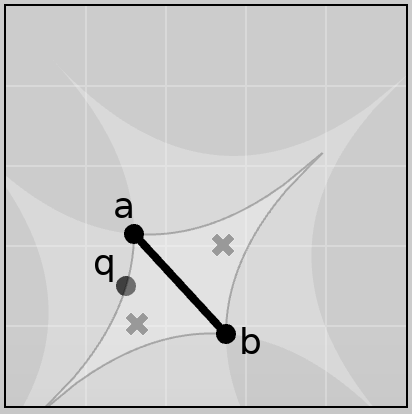
\includegraphics[width=0.48\linewidth]{figs/chap7/bskeleton.png}
    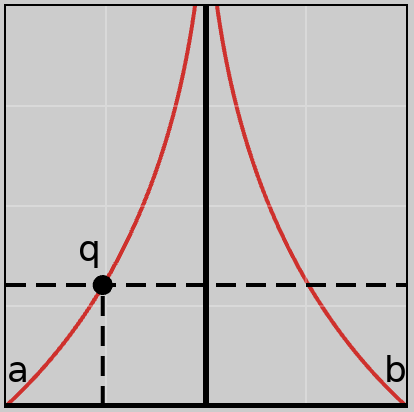
\includegraphics[width=0.48\linewidth]{figs/chap7/bskeletonParameter.png}
    \caption{Left: An example of a two-dimensional edge defined by points $a$ and $b$.
    %
    We test whether the query point $q$ is interior to the region $R_{\beta,p}(a,b)$.
    %
    $R_{\beta,p}(a,b)$ is defined as the intersection of two $p$-balls whose center points are shown as grey x's.
    %
    Right: The edge test can be reformulated as a 1-dimensional problem where we compare $q$'s $L^2$-distance to $ab$ and the equation of the $p$-ball centered at a distance determined by $\beta$ from the edge's midpoint.}
    \label{fig:gabriel_p_shapes}
\end{figure}

\subsubsection{Discretized Empty Region Graph Algorithm}
\label{sec:gpu_bp_discrete}

The one-dimensional function given in Equation~\ref{eq:beta_parameterization} has only one dependence on the length of $ab$.
%
Thus, we can precompute the template function offline and scale it accordingly for each edge in our GPU kernel.
%
This leads us to a discretized algorithm where the fidelity of the precomputed approximation is a function of the number of discrete steps $s$ used to store the function.
%
Note, that since the function is symmetric about the midpoint, we can devote all $s$ samples to one half of the shape, as noted by the domain of Equation~\ref{eq:beta_parameterization}.

Furthermore, this simplifciation allows us to substitute any arbitrarily complex kernel function for the $L^p$-balls presented thus far.
%
For example, in Figure~\ref{fig:discrete_beta}, we demonstrate the use of a several different common kernel functions including a properly scaled Gaussian, Epanechnikov, cosine, quartic, and tricubic functions on a set of 20 CVT sampled points in 2D.
%
We compare these results with the standard $L^p$ norm example and note that the results are unique for each realized graph.

\begin{figure}
    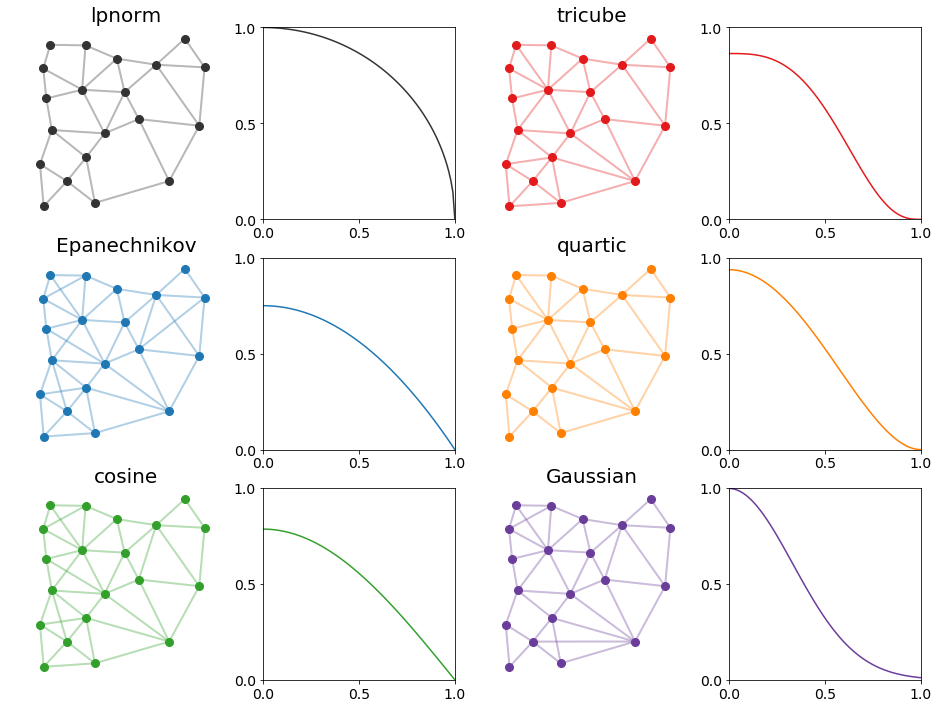
\includegraphics[width=\linewidth]{figs/chap7/beta_shapes.png}
    \caption{Using discretization to precompute a template function, we can employ arbitrarily complex functions without incurring any additional overhead cost.
    %
    Here we demonstrate using several different common kernel functions and visual the resulting graph.
    %
    The color-coordinated adjacent line plots of each graph show the shape of the template functions used.}
    \label{fig:discrete_beta}
\end{figure}

\subsubsection{Probabilistic Empty Region Graphs}

Our method for computing probabilistic $\beta_p$-skeletons is similar in spirit to the methodology used by Correa and Lindstrom's stochastic empty region graph in that we correspond an edge's probability to the largest minimum amount of distance any empty region violating neighbors of its endpoints need to move to be placed outside of its empty region.
%
\DPM{Why is this better/different?}
%
We differ in how we parameterize the problem.
%
Correa and Lindstrom utilize an inner and outermost region, $R_{\alpha_{min}}$ and $R_{\alpha_{max}}$ where probability uniformly increases from 0 to 1 over $\alpha \in [\alpha_{min},\alpha_{max}]$ over this region.
%
Any edge with a neighbor inside $R_{\alpha_{min}}$ will have probability 0 and any edge with no neighbors inside of $R_{\alpha_{max}}$ will have probability 1.

We instead utilize a logistic function in order to adjust the steepness of the probability fall-off and do not express set minimum and maximum regions.
%
Given a neighbor $q$'s projection onto $ab$, $t_q$, its $L^2$ distance from $ab$, $d_{t_q}$, and $D(\cdot)$ from Equation~\ref{eq:beta_parameterization}, we define an edge's probability with respect to $q$ as:

\begin{equation}
\label{eq:probabilistic_beta}
    l(t_q) = \left(1 + e^{-\frac{k}{D(2|t_q - 0.5|)}\left(d_{t_q}-D(2|t_q - 0.5|)\right)}\right)^{-1}
\end{equation}

Thus, the probability of an edge is the minimum of Equation~\ref{eq:probabilistic_beta} for all neighbors considered for an edge's endpoints.
%

An example probabilistic graph is shown in the rightmost image of Figure~\ref{fig:probabilistic_beta}.
%
The leftmost plot shows the shape of the specific logistic function, and the center image shows the probability as a function of distance from a specific edge.
%
Here solid lines represent probability above $75\%$, dashed-dotted lines represent probability above $50\%$, dashed lines represent probability above $25\%$, and dotted lines represent edges with $<25\%$ probability.

\begin{figure}
    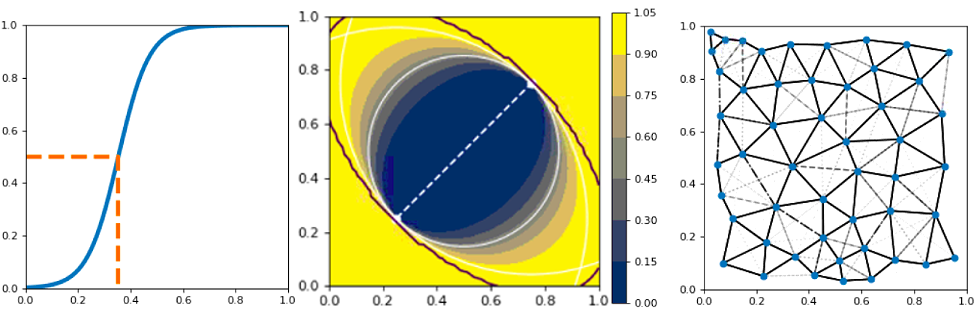
\includegraphics[width=\linewidth]{figs/chap7/probabilistic_beta.png}
    \caption{An example of a probabilistic Gabriel graph.
    %
    The left plot shows the logistic function used to determine the steepness by which the probability will fall off as a distance from the canonical empty region boundary (in this case the white circle of the middle image).
    %
    The orange line indicates the 50\% probability point.
    %
    The middle image shows the probability as a colormap under the edge.
    %
    The right image visualizes the graph using different line styles to denote probability.
    %
    Solid lines >75\%, dashed-dotted lines > 50\%, dashed > 25\%, dotted < 25\%.}
    \label{fig:probabilistic_beta}
\end{figure}

\subsection{Cone Graphs}

Consider we want to compute either an $m$-Yao or $m$-$\Theta$-Graph where $m$ is the number of points per cone.
%
For a given query point, we initialize a counting array of size $c$ zeros.
%
We then iteratively compute the $i$th nearest neighbor's cosine similarity to each of the $c$ axes and determine which cone this neighbor belongs to by taking the maximum.
%
If the counting array index associated to this cone is less than $m$, we increment the count and keep this edge.
%
Otherwise, we invalidate this edge by replacing it with a $-1$.
%
For the Yao graph, we make use of the ordered $k$-nearest neighbors provided by our knn query structure.
%
Since the $k$-nearest neighbors for each point are given in order of increasing distance to the query point we are guaranteed to fill each conic with the the closest neighbors for the Yao graph.

If instead we are computing the $\Theta$ graph, we must reorder the points based on their projected distance which we have already computed in order to determine the closest axis.
%
Alternatively, we could use an auxiliary data structure to maintain the $m$ closest distances for each axis and process the neighbors sequentially.
%
Thus, we can incur a $\bigO(k \log k)$ sort operation per query point/thread to sort the $k$ neighbors in increasing distance to their respective axis, or add a local $\bigO(cm)$ storage per thread to store the $m$ closest distances for each of the $c$.
%
For most practical settings, $m$ is set to 1 or 2 and we seek to use a minimal $c$ that achieves the fidelity we want, whereas $k$ is often maximized in order to start with the most information possible for pruning.
%
On the other hand, the sorts can be done in parallel for each query.
%
% We examine both implementations in Section~\ref{exp:performance}.
% %
% \dpm{I have not implemented this. Make sure there are no devils in the details.}

\subsubsection{Probabilistic Cone Graphs}

Note that the cone graphs are largely dependent on the generated directions.
% %
% The $\Theta$-graph especially can select a completely different set of neighbors with only a small perturbation in angle of directions.
% %
% Figure~\ref{fig:cone_graphs} demonstrates how rotating the axes with the same point set yields different results for both the Yao and $\Theta$-graph.
% %
% In this case, two of eight Yao neighbors have changed, and seven of
% eight $\Theta$ neighbors have changed.
%
Exploting this fact, one way to generate a probabilistic result is to use several different random seeds for the CCVT sample generation.
%
The result is a collection of different graph realizations.
%
We then associate probability to an edge equal to the proportion of realizations in which it occurs.
%
The justification for doing this is that stable edges will be robust to the actual cones selected.

% \begin{figure}
%     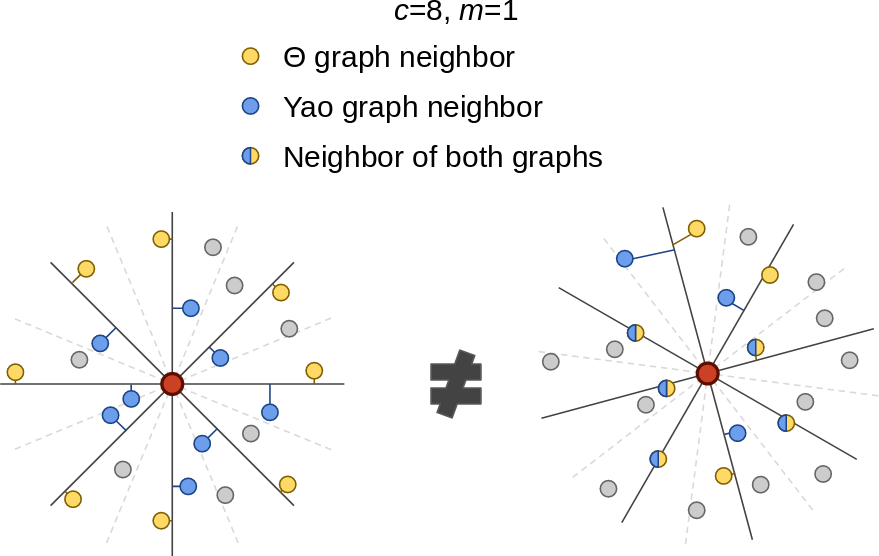
\includegraphics[width=\linewidth]{figs/chap7/cone_graphs.png}
%     \caption{Two examples are shown for determining neighbors of the
%     same central red query point.
%     The solid lines represent the $8$ cone axes which are perturbed
%     between the two images. Blue and yellow dots represent neighbors
%     identified by the Yao and $\Theta$ graphs, respectively. Dotted
%     lines represent cone boundaries and grey points are points that
%     are not neighbors to the query point under either graph
%     representation. \dpm{Re-do this image with corrected $\theta$ graph.}}
%     \label{fig:cone_graphs}
% \end{figure}

\section{Quality Measueres}
\label{sec:graph_quality_measures}
An open question to consider is what makes a ``good'' graph?
%
Though the answer largely depends on the application, we attempt to generalize properties from the topological and geometric properties of the dataset as well as our target applications and come up with five measures applicable in low dimensions to evaluate different proximity graphs.
%
For higher dimensions, we will rely on an application-specific study to perform evaluations.

The five measures are listed below with a brief justification for each.
%
These five measures basically capture the consistency in topology and geometry between the graph and the underlying data distribution.
%
To evaluate the constructed graph, two of them, number of crossing edges and average induced polygon area, are computed from the properties of the graph and compared.
%
To evaluate the consistency in the graph representation with respect to the data representation, three of the them, number of connected component, $\alpha$-shape coverage and total out-of-bound length, rely on both the constructed graph and the computation of an $\alpha$-shape~\cite{EdelsbrunnerKirkpatrickSeidel1983}, where we tune $\alpha$ for each chosen dataset in order to extract a tight hull of the distribution of points in the plane.
%
Examples of the point distributions and their extracted shapes are given in Figure~\ref{fig:shapes}.

\paragraph{\textbf{Crossing Edge Count}} %Crossing edges is considered a negative in our graphs.
%
Crossing edges in a way encode redundant information by over-connecting the graph and can actually create contradictory information in terms of interpolation.
%
For example, in the application of scalar field topology, the presence of crossing edges can actually result in crossing integral lines which violates one of the fundamental tenets for analysis.
%
The number of crossing edges is computed and used as a negative measure in building a good graph.

\paragraph{\textbf{Average Induced Polygon Area}} If crossing edges represent a negative characteristic of an over-connected graph, then the average empty space area represents the other side of the spectrum, an under-connected graph.
%
One way to compute the amount of empty space in a graph is to induce a polygonization of the graph by including all faces where the edges of our graph form a closed polygon.
%
%Such a polygonization will have no edges on the interior of any polygon, thus we minimize the area of every polygon in our induced polygonization.\dw{rewrite this sentence}
%
By computing the average area of this set of polygons, we get a sense of how much empty space there is in the graph's interior.
%
The larger the area of the polygons, the more prone the graph is to being sparse.
%
The problem with this measure in isolation is that it will tend to favor under connected graphs that have no closed polygons and so will report a minimal value of zero for the average area.
%
We counterbalance this measure with the number of crossing edges and the next measure which ensures the topological consistency.

\paragraph{\textbf{Connected Components}} We compute the absolute difference between the  umber of connected components of the alpha shape and the number of connected components of the graph.
%
This will penalize both under-connected graphs, which create many small and spurious components, and over-connected graphs, which fail to capture the intrinsic shape of the data.

\paragraph{\textbf{$\alpha$-shape Coverage}} Using the induced polygonization from above, we can also compute how well that polygonization covers the shape of the data.
%
For this we perform an intersection operation between the induced polygonization and the $\alpha$-shape.
%
We then compute the total area of this intersection divided by the total area of the $\alpha$-shape.
%
In this way, a value of one represents complete coverage of the shape and a value of zero means no coverage.

\paragraph{\textbf{Total Out of Bounds Length}} To compensate for the previous measure, where a fully connected graph will always report a coverage of one, we also compute the lengths of edges outside the $\alpha$-shape.
%
% The problem with the previous measure is that a fully connected graph will always report a coverage of one.
%
The coverage measure can in some sense be thought of as a recall measure, showing how much of the total shape of the data can be recovered.
%
Thus we also need to couple that with a precision measure that penalizes edges that fall outside of the $\alpha$-shape.
%
To satisfy this criteria, we chose to accumulate the total length of edges outside the $\alpha$-shape.
%
Note that we perform a difference operator on all edges, such that we only include the portions of edges that fall outside of the given $\alpha$-shape.

\DPM{Explain negation below.}

In order to digest these five measures, we normalize them over their respective ranges and perform linear scalarization to create a composite measure that we can use to optimize the parameters of each graph type.

\begin{equation}
    M_{composite} = \sum_{i=1}^5 M_iw_i
\end{equation}

For the experiments in this paper we use $w_i=1$.

\section{Analysis}

\DPM{Add preamble here.}

\subsection{Supergraph Saturation}

\DPM{Include study from scalable topology paper.}

\subsection{Performance Analysis}

In this section, we compare the performance of the existing serial algorithm provided by NGL to our GPU implementation.
%
Both libraries have been modified to accept a pre-computed $k$-nearest neighbor graph for pruning, and therefore timing results do not include the computation of the $k$-nearest neighbor graph.
%
We first investigate each library's ability to reconstruct both a strict and relaxed Gabriel graph in dimensions ranging from two to ten dimensions on small (ten thousand) to moderate (one million) sized problems.
%
We show results for a uniform, random point sampling strategy, but the specific distribution should not significantly impact the running time of either implementation, our tests support this claim as similar performance is acheived on other strategies such as a CVT, a Latin Hypercube design, and a normally distributed point set of the same size.
%
The results reported in Figure~\ref{fig:performance} have been averaged over ten trials with error bars showing one standard deviation.
%
The error bars are hardly visible demonstrating that the deviations in performance for the different algorithms are indeed statistically significant.
%
The top row shows results for the strict Gabriel graph and the bottom row shows results for the relaxed Gabriel graph.
%
The number of neighbors used in the underlying $k$-nn graph varies commensurate with the dimension, thus performance is as much a factor of $k$ as it is dimensionality in these cases.
%
We see for smaller problems and lower dimensions, both implementations offer competitive speeds, but as the dimensionality and $k$ grow, our implementation is able to offer even more speed-up.
%
Furthermore the discretized version can add modest improvement to the GPU algorithm with only minor differences in the resulting graph.
%
\DPM{Demonstrate what is meant by a ``minor'' difference}.

\begin{figure}
    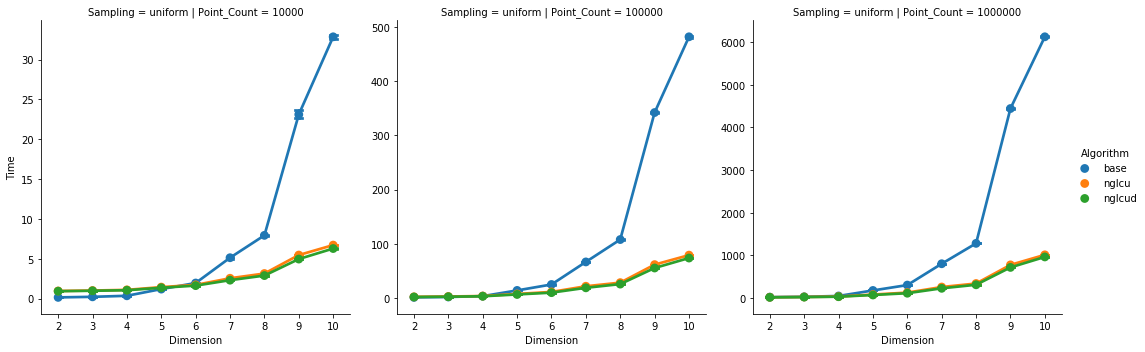
\includegraphics[width=0.8\linewidth]{figs/chap7/strict_performance_d.png}
    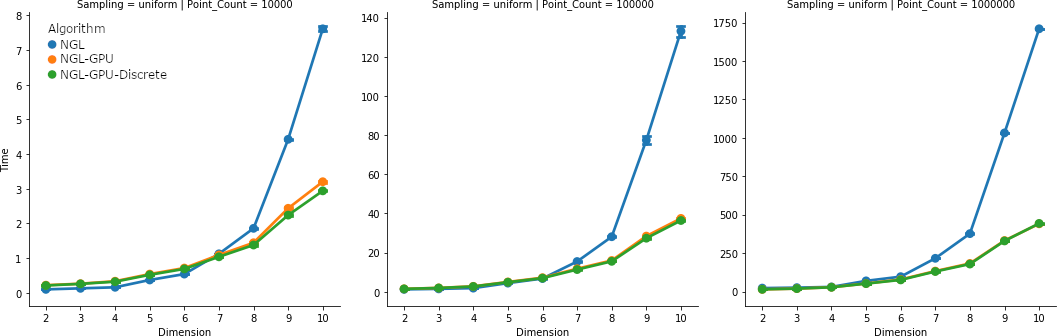
\includegraphics[width=0.8\linewidth]{figs/chap7/relaxed_performance_d.png}
    \caption{We report the performance of NGL (blue) and two of our GPU
    implementations (standard - orange, and discrete - green) by
    evaluating time as a function of the dimensionality. For the
    dimensionalities listed we use the following values for $k$ in
    pruning: $d < 5$, $k=100$, $d < 7$, $k=200$, $d < 9$, $k=300$, and
    otherwise $k=500$. From left to right in both rows, the sample sizes
    are 10000, 100000, 1000000.}
    \label{fig:performance}
\end{figure}

\begin{itemize}
    \item \DPM{Next show an example where the algorithm does not fit entirely on the GPU, go to from 10 million to 1 billion in 2 to 5 dimensions and fix the query size to be sure.}
    \item \DPM{Compare to ourselves how long different graphs take to generate: yao, theta, $\beta=0.5, 1, 1.5, 2$ for $p=0.5, 1, 1.5, 2, 4$}
    \item \DPM{Need CUDA implementation of $\Theta$}
    \item \DPM{Compare computation of $\Theta$-graph using sort in place and extra data array for storage.}
\end{itemize}

\subsection{2D Graph Quality Measures}

Here we evaluate the measures defined in Section~\ref{sec:graph_quality_measures}
on various two dimensional distributions using different sized sample sets.

\begin{figure}[!ht]
  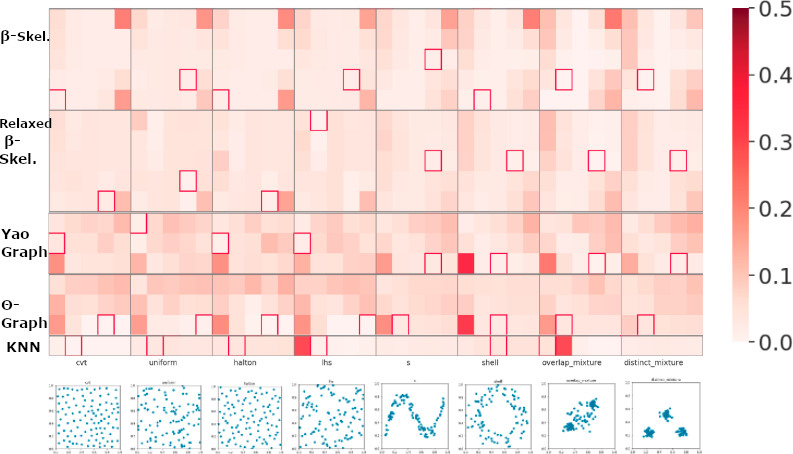
\includegraphics[width=\linewidth]{figs/chap7/Combined5graphs.png}
  \caption{A graph quality heatmap based on aggregation of five graph quality measures on five proximity graphs for eight different distributions.
  %
  The optimal parameter setting for each graph is highlighted.}
  \label{fig:teaser}
\end{figure}

Figure~\ref{fig:teaser} shows the results of our five graphs on nine distributions of points.
%
The heatmap shows the values of $M_{composite}$ computed for eight different data distributions and five different different graphs.
%
Each cell also contains multiple sub-cells denoting the  $M_{composite}$ value for that specific parameter setting, where the optimal setting for each graph was denoted by the highlighted cell.
%
According to the quality measure shown in Figure~\ref{fig:teaser}, there is no universal optimal parameters for different distributions and sample sizes.

\begin{figure}
    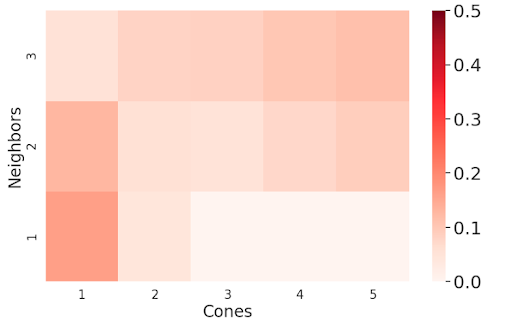
\includegraphics[width=0.48\linewidth]{figs/chap7/yao_heatmap_2.png}
    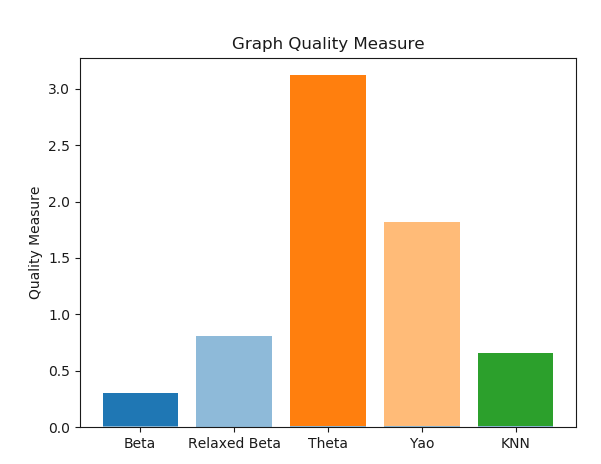
\includegraphics[width=0.48\linewidth]{figs/chap7/optimal_quality_measures.png}
    \caption{Analysis of five different graphs using our graph quality measures.
    %
    Left: We evaluate a single graph in isolation by looking at a heatmap of the aggregate quality measures for different parameter settings.
    %
    Right: Once an optimal setting is decided we compare it with aggregate quality measures of the other graphs.
    %
    In this case, the strict $\beta$-skeleton reports the best aggregate quality as determined by the lowest possible score.}
    \label{fig:graph_svm}
\end{figure}

\subsection{Topological Accuracy and Stability}

\DPM{Include TopoInVis study?}

\begin{figure}
    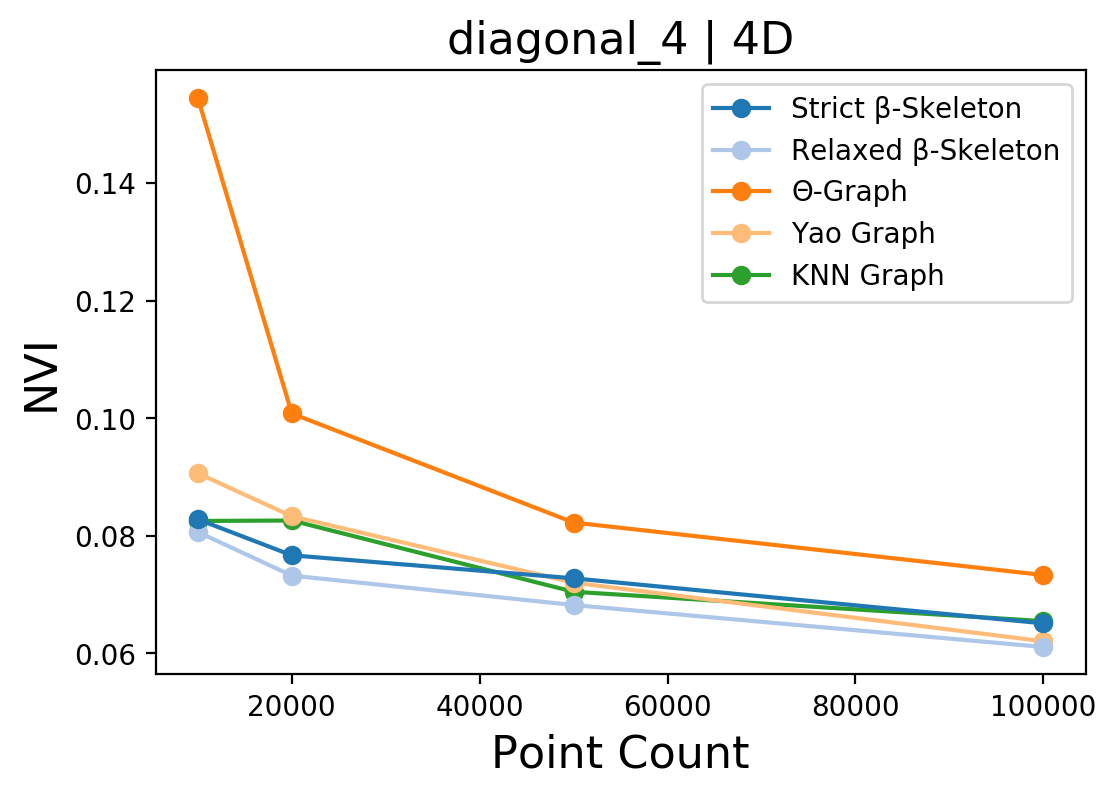
\includegraphics[width=0.48\linewidth]{figs/chap7/diagonal_4_nvi.png}
    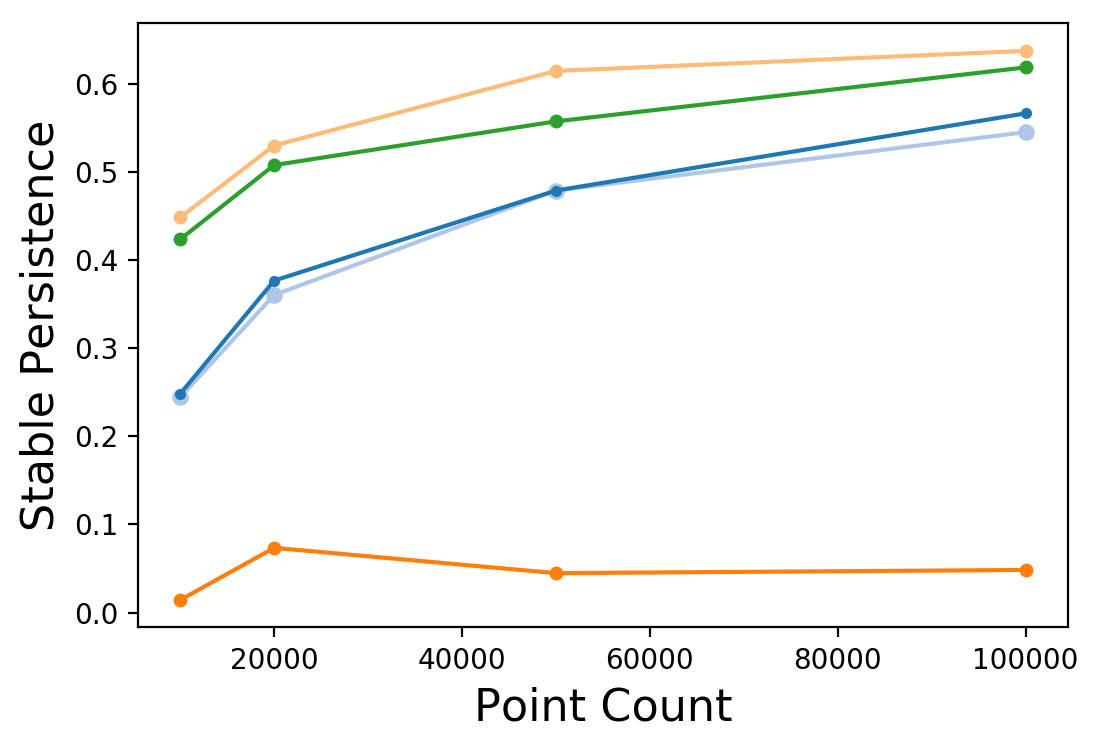
\includegraphics[width=0.48\linewidth]{figs/chap7/diagonal_4_stability.png}
    \caption{Analysis of five different graphs  under the topological setting.
    Left: We then repeat the process of tuning for our topological problem and report the NVI of the best-in-class for each graph.
    %
    Right: Along with NVI we report the persistence stability that each graph is able to maintain the correct partition.}
    \label{fig:graph_topo}
\end{figure}

\subsection{SVM Classification Enhancement}

SVMs were introduced in Section~\ref{sec:svm}.
%
Zhang and King~\cite{ZhangKing2002a, ZhangKing2002b} determined that by pre-processing a dataset with an appropriate graph structure (in this case, they chose a $\beta$-skeleton), they were able to drastically reduce the training set size thus reducing computation time, while maintaining simliar accuracy.
%
Goto et al.~\cite{GotoIshidaUchida2015} performed a similar study using the relative neighbor graph and identifying what they called \textit{bridge vectors}.
%
However, the first example of using proximity graphs to reduce training sizes on classification problems dates back to 1981 where Bhattacharya et al. used the technique on a nearest neighbor classifier~\cite{BhattacharyaPoulsenToussaint1981}.

The idea for SVMs takes advantage of the fact that the SVM is made up of \textit{support vectors} that describe the boundaries of separate classes.
%
By preprocessing the data with a proximity graph and only including the endpoints of edges that belong to separate classes, we prune away much of the uninformative data while with high probability keeping data points that will be the support vectors the model is seeking.
%
We seek to replicate results on two classification datasets.
%
The first is a handwritten letter analysis publicly available from the UCI Machine Learning Repository~\cite{DuaGraff2017} where image data is vectorized and the goal is to determine the letter that each image represents.
%
The latter is studying a station blackout scenario for nuclear power plant safety simulation~\cite{MaljovecLiuWang2015}.
%
In this study, we study the recovery procedure from an accident situation and the goal is to classify whether the plant can be safely recovered before the core reaches an irrecoverable temperature.
%
The dimensionality of the examples are 16 and 12, respectively, and each is made up of roughly 20000 point samples.

The results of this study are shown in the bottom row of images of Figure~\ref{fig:applications} where we show a Pareto front of parameter settings for each graph trading off data reduction with accuracy.
%
Note, the scale of the horizontal axis in both images varies drastically.
%
For the nuclear dataset (right), the upper left point of the strict $\beta$-skeleton indicates that we are able to drastically reduce the data size with only minimal detriment to the accuracy.
%
For the handwriting dataset, the strict $\beta$-skeleton is still Pareto dominant, but the degradation in performance is much worse and the other methods are more competitive in the range of accuracy most would deem acceptable.

\begin{figure}
    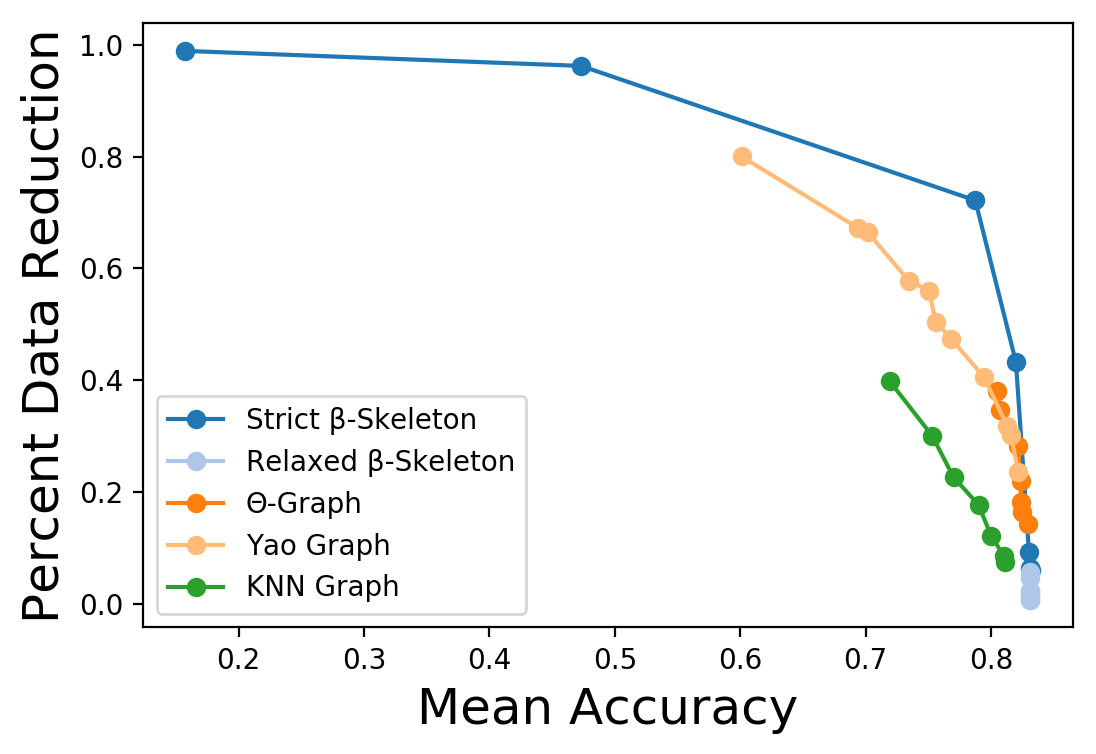
\includegraphics[width=0.48\linewidth]{figs/chap7/pareto_letters.png}
    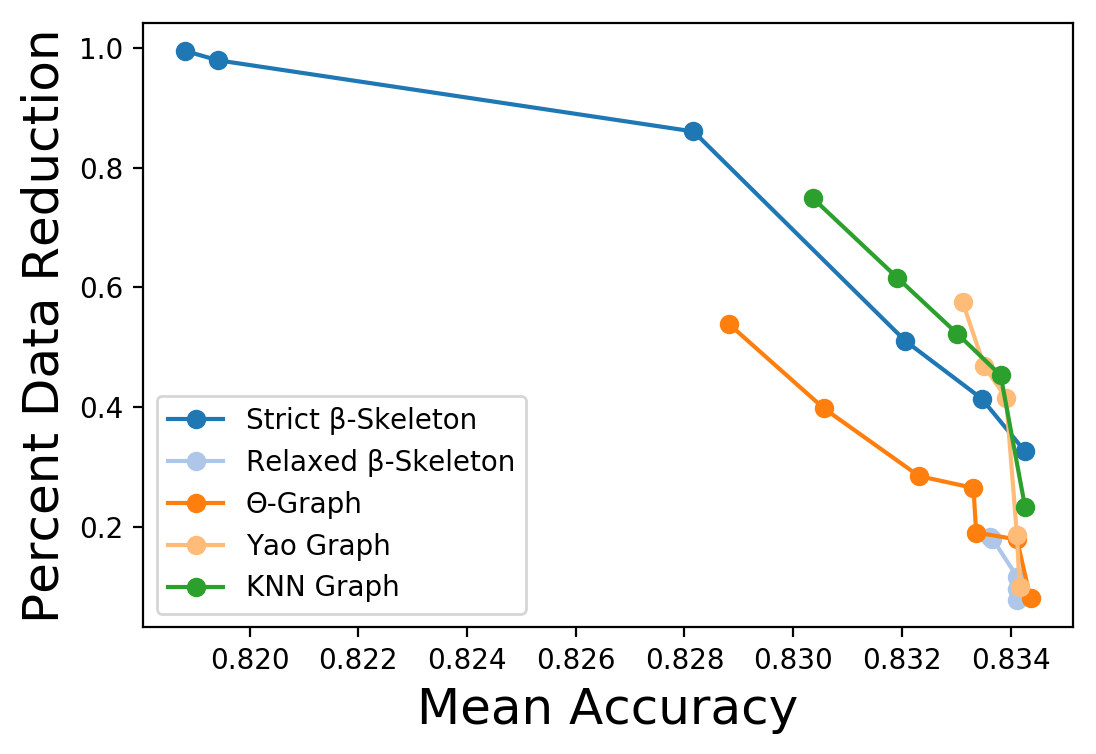
\includegraphics[width=0.48\linewidth]{figs/chap7/pareto_sbo.png}
    \caption{Analysis of five different graphs for two classification datasets.
    %
    Left: For the SVM evaluation, we report a Pareto front over the handwritten dataset.
    %
    Right: We similarly report results for the station blackout dataset.}
    \label{fig:graph_svm}
\end{figure}